\documentclass[conference]{IEEEtran}
\IEEEoverridecommandlockouts

\usepackage{cite}
\usepackage{amsmath,amssymb,amsfonts}
\usepackage{graphicx}
\usepackage{textcomp}
\usepackage{xcolor}
\usepackage{booktabs}
\usepackage{array}
\usepackage[utf8]{inputenc}
\usepackage[T1]{fontenc}
\graphicspath{{figs/svm_rbf/}}

\def\BibTeX{{\rm B\kern-.05em{\sc i\kern-.025em b}\kern-.08em
    T\kern-.1667em\lower.7ex\hbox{E}\kern-.125emX}}

\begin{document}

\title{Classificação Supervisionada de Áreas Queimadas\\
com SVM Kernel RBF e Imagens Landsat~8/9}

\author{
  \IEEEauthorblockN{Autor}
  \IEEEauthorblockA{
    \textit{Reconhecimento de Padrões}\\
    Sensoriamento Remoto Orbital $\cdot$ Landsat~8/9\\
    Cenas 220\_075, 221\_074 e 222\_074 $\cdot$ Agosto de 2024
  }
}

\maketitle

\begin{abstract}
Uma Máquina de Vetores de Suporte (SVM) com kernel RBF foi treinada com
amostras rotuladas de uma cena Landsat para classificar cada pixel em
\textbf{Queimado} ou \textbf{Não Queimado}. Usando 10~atributos espectrais
extraídos de imagens pré e pós-queimada, o modelo generalizou com alto
desempenho para duas cenas geograficamente independentes — demonstrando que
a assinatura espectral de queimadas é robusta o suficiente para ser aprendida
por um único conjunto de treinamento. Os hiperparâmetros de regularização
($C$) e forma do kernel ($\gamma$) foram otimizados via Optuna (50~tentativas),
atingindo $F_1 > 99\%$ e AUC-ROC~$= 1{,}000$ nos testes cegos.
\end{abstract}

\begin{IEEEkeywords}
área queimada, SVM, kernel RBF, Optuna, Landsat, sensoriamento remoto,
generalização espacial, teste cego.
\end{IEEEkeywords}

%=====================================================================
\section{Problema, Entradas e Saída do Modelo}

\textbf{Objetivo:} dado um pixel de uma imagem de satélite, determinar se
ele pertence a uma área que sofreu queimada recente ou não —
\textbf{classificação binária supervisionada pixel a pixel}.

A Tabela~\ref{tab:io} resume o fluxo de entrada e saída do modelo.

\begin{table}[!t]
  \caption{Entradas e saídas da SVM RBF}
  \label{tab:io}
  \centering
  \begin{tabular}{ll}
    \toprule
    \textbf{ENTRADA} & \textbf{SAÍDA} \\
    \midrule
    10 atributos por pixel & Classe por pixel \\
    Bandas B4, B5, B7 & 1 = Queimado \\
    Índices NDVI e NBR & 0 = Não Queimado \\
    (pré e pós-queimada) & + mapa de probabilidade \\
    \bottomrule
  \end{tabular}
\end{table}

%=====================================================================
\section{Metodologia}

\subsection{Dados e Estratégia de Treino/Teste}

Foram usadas três cenas Landsat~8/9 localizadas no estado de São Paulo
(agosto de 2024), cada uma com um par de imagens pré e pós-queimada:

\begin{itemize}
  \item \textbf{220\_075} — cena de \textbf{treino e validação}, com máscara
        de referência (\textit{ground-truth}) disponível;
  \item \textbf{221\_074} e \textbf{222\_074} — cenas de \textbf{teste cego},
        geograficamente distintas, nunca vistas pelo modelo durante o treino.
\end{itemize}

Adicionalmente, imagens com cobertura de nuvens foram incluídas no treino
como amostras da classe \textit{não queimada}, aumentando a robustez do
modelo a condições de nebulosidade.

\subsection{Atributos Espectrais}

Para cada pixel, cinco atributos são extraídos da imagem pré-queimada e
outros cinco da pós-queimada, formando um vetor de 10~features.
A Tabela~\ref{tab:features} descreve cada atributo.

\begin{table}[!t]
  \caption{Atributos espectrais utilizados}
  \label{tab:features}
  \centering
  \begin{tabular}{lll}
    \toprule
    \textbf{Atributo} & \textbf{O que mede} & \textbf{Por que importa} \\
    \midrule
    B4 (Red) & Reflectância no vermelho
             & Aumenta após queimada \\
    B5 (NIR) & Reflectância no IV próximo
             & Cai após destruição da vegetação \\
    B7 (SWIR2) & Reflectância no IV onda curta
               & Alto em solo exposto e queimado \\
    NDVI & Índice de vegetação
         & Queda indica perda de cobertura \\
    NBR  & Índice de queimada
         & Principal discriminador de cicatrizes \\
    \bottomrule
  \end{tabular}
\end{table}

\subsection{Como a SVM RBF Funciona}

\begin{enumerate}
  \item \textbf{Treinamento}: a SVM aprende uma fronteira de decisão
        não-linear no espaço dos 10~atributos, separando pixels queimados
        dos não queimados. Apenas as amostras mais próximas da fronteira
        — os \textit{vetores de suporte} — definem o modelo final.
  \item \textbf{Otimização}: os hiperparâmetros de regularização ($C$) e
        forma do kernel ($\gamma$) foram ajustados automaticamente via
        \textbf{Optuna} (50~tentativas, TPE Sampler), maximizando o F1 em
        validação cruzada.
  \item \textbf{Inferência}: o modelo classifica a cena de teste inteira em
        lotes, produzindo a classe binária e a probabilidade de cada pixel.
\end{enumerate}

A função de decisão do kernel RBF é dada por:

\begin{equation}
  K(\mathbf{x}, \mathbf{x}') = \exp\!\left(-\gamma \|\mathbf{x} - \mathbf{x}'\|^2\right)
  \label{eq:rbf}
\end{equation}

onde $\gamma$ controla a largura da função radial. Valores altos de $\gamma$
criam fronteiras mais curvilíneas; valores baixos produzem fronteiras mais
suaves.

%=====================================================================
\section{Dados de Entrada}

Na composição falsa-cor B7/B5/B4, as áreas queimadas aparecem em vermelho
intenso — reflexo da alta reflectância em SWIR2 e colapso do NIR. Essa
separabilidade visual é o que a SVM aprende a capturar numericamente no
espaço de 10~atributos espectrais, como ilustra a Fig.~\ref{fig:falsa_cor}.

\begin{figure}[!t]
  \centering
  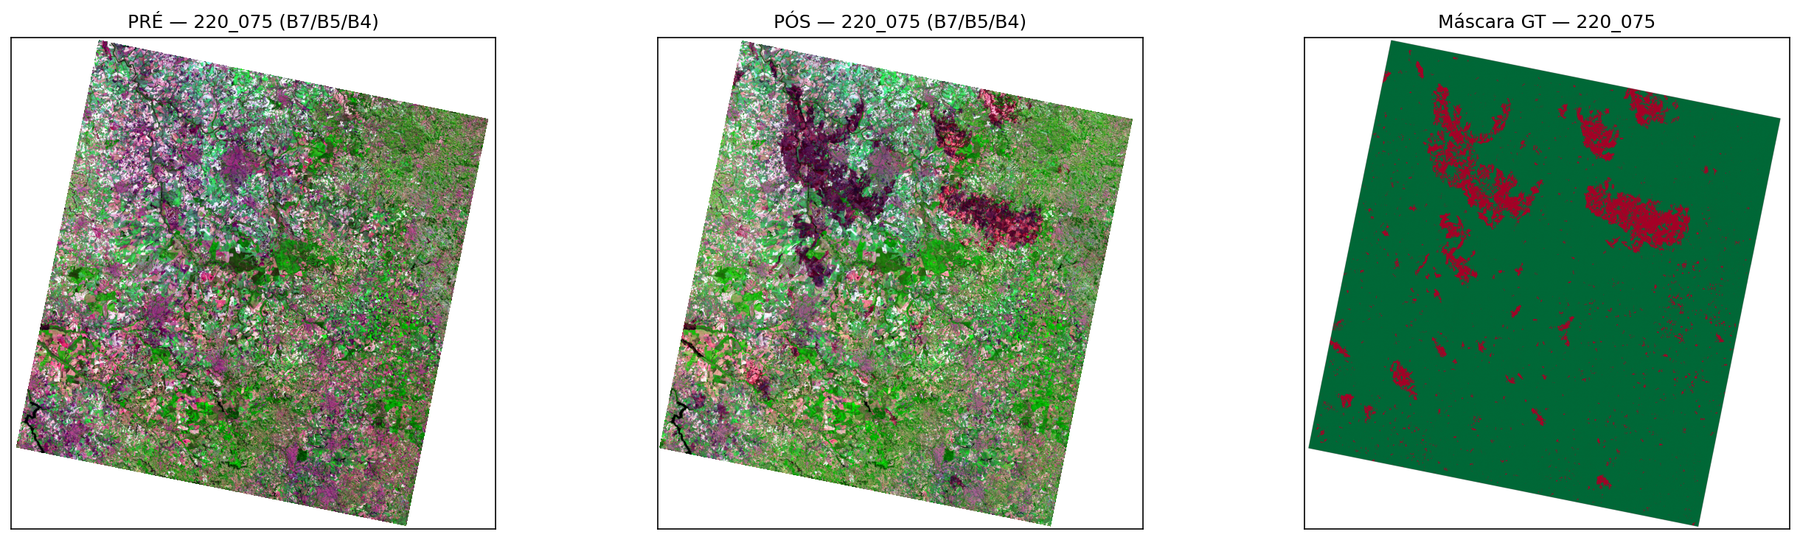
\includegraphics[width=\columnwidth]{fig_falsa_cor.png}
  \caption{Cena de treino 220\_075: composição falsa-cor pré-queimada (esq.),
           pós-queimada (centro) e máscara \textit{ground-truth} (dir.).
           Áreas queimadas em vermelho na imagem pós-queimada.}
  \label{fig:falsa_cor}
\end{figure}

%=====================================================================
\section{Resultados}

\subsection{Otimização de Hiperparâmetros}

A busca automática pelo Optuna encontrou rapidamente a região de melhor
desempenho no espaço de configurações. A maioria dos melhores resultados
concentrou-se em valores altos de regularização ($C$), indicando que o
problema possui fronteira de decisão complexa que se beneficia de menor
penalização da margem. A Fig.~\ref{fig:optuna} mostra a convergência do F1.

\begin{figure}[!t]
  \centering
  
\includegraphics[width=\columnwidth]{fig_optuna.png}
  \caption{Busca de hiperparâmetros — Optuna (50~tentativas): evolução do
           melhor F1 acumulado (esq.) e distribuição dos pontos testados no
           espaço $C \times \gamma$ (dir.), coloridos pelo F1 obtido.}
  \label{fig:optuna}
\end{figure}

\subsection{Desempenho nas Cenas de Teste}

O modelo foi avaliado em duas cenas completamente independentes.
A Tabela~\ref{tab:results} resume os resultados — todos os conjuntos
atingiram $F_1$ acima de 0,98 e AUC-ROC perfeita.

\begin{table}[!t]
  \caption{Desempenho da SVM RBF em todos os conjuntos}
  \label{tab:results}
  \centering
  \setlength{\tabcolsep}{4pt}
  \begin{tabular}{lcccc}
    \toprule
    \textbf{Conjunto} & \textbf{Acurácia} & \textbf{Precisão}
                      & \textbf{Recall} & \textbf{F1} \\
    \midrule
    Treino (50k amostras)     & 99,96\% & 98,69\% & 100,00\% & \textbf{99,34\%} \\
    Validação (12M pixels)    & 99,85\% & 98,40\% &  99,76\% & \textbf{99,07\%} \\
    Teste cego 221\_074 (40M) & 99,91\% & 98,60\% &  99,64\% & \textbf{99,12\%} \\
    Teste cego 222\_074 (40M) & 99,88\% & 96,83\% &  99,30\% & \textbf{98,05\%} \\
    \bottomrule
    \multicolumn{5}{l}{AUC-ROC $= 1{,}000$ em todos os conjuntos.}
  \end{tabular}
\end{table}

\subsection{Matrizes de Confusão}

A Tabela~\ref{tab:cm221} e a Tabela~\ref{tab:cm222} apresentam as matrizes
de confusão para as duas cenas de teste cego.

\begin{table}[!t]
  \caption{Matriz de Confusão — Teste Cego 221\_074}
  \label{tab:cm221}
  \centering
  \begin{tabular}{lcc}
    \toprule
    & \textbf{Pred.\ Não Queimado} & \textbf{Pred.\ Queimado} \\
    \midrule
    \textbf{Real Não Queimado} & 38.143.005 (TN) & 27.725 (FP) \\
    \textbf{Real Queimado}     &      2.669 (FN) & 720.603 (TP) \\
    \bottomrule
  \end{tabular}
\end{table}

\begin{table}[!t]
  \caption{Matriz de Confusão — Teste Cego 222\_074}
  \label{tab:cm222}
  \centering
  \begin{tabular}{lcc}
    \toprule
    & \textbf{Pred.\ Não Queimado} & \textbf{Pred.\ Queimado} \\
    \midrule
    \textbf{Real Não Queimado} & 38.853 (TN) & 8.177 (FP) \\
    \textbf{Real Queimado}     &    8.571 (FN) & 1.180.989 (TP) \\
    \bottomrule
  \end{tabular}
\end{table}

A curva ROC perfeita (AUC~$= 1{,}000$) confirma separabilidade completa
entre as classes no espaço de probabilidade, como ilustra a Fig.~\ref{fig:cm_roc}.

\begin{figure}[!t]
  \centering
  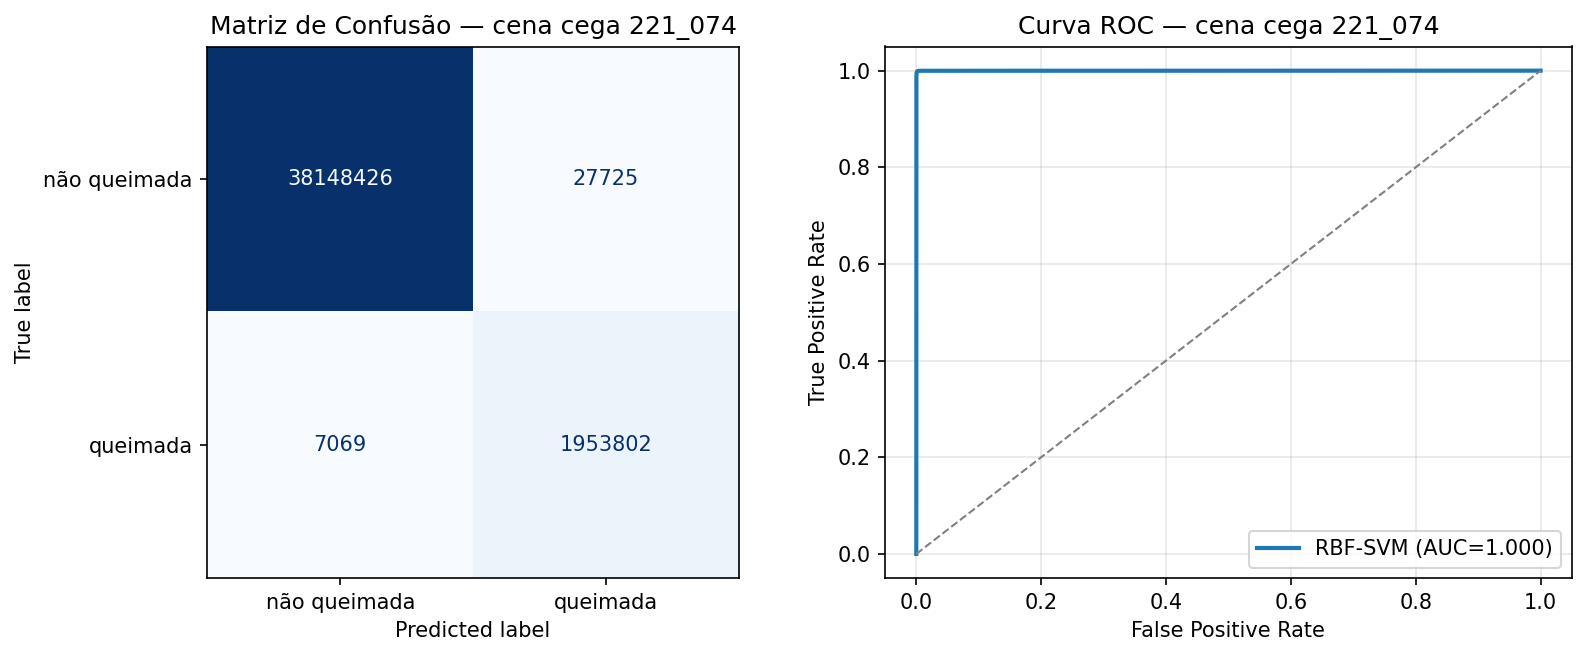
\includegraphics[width=\columnwidth]{fig_cm_221.png}\\[4pt]
  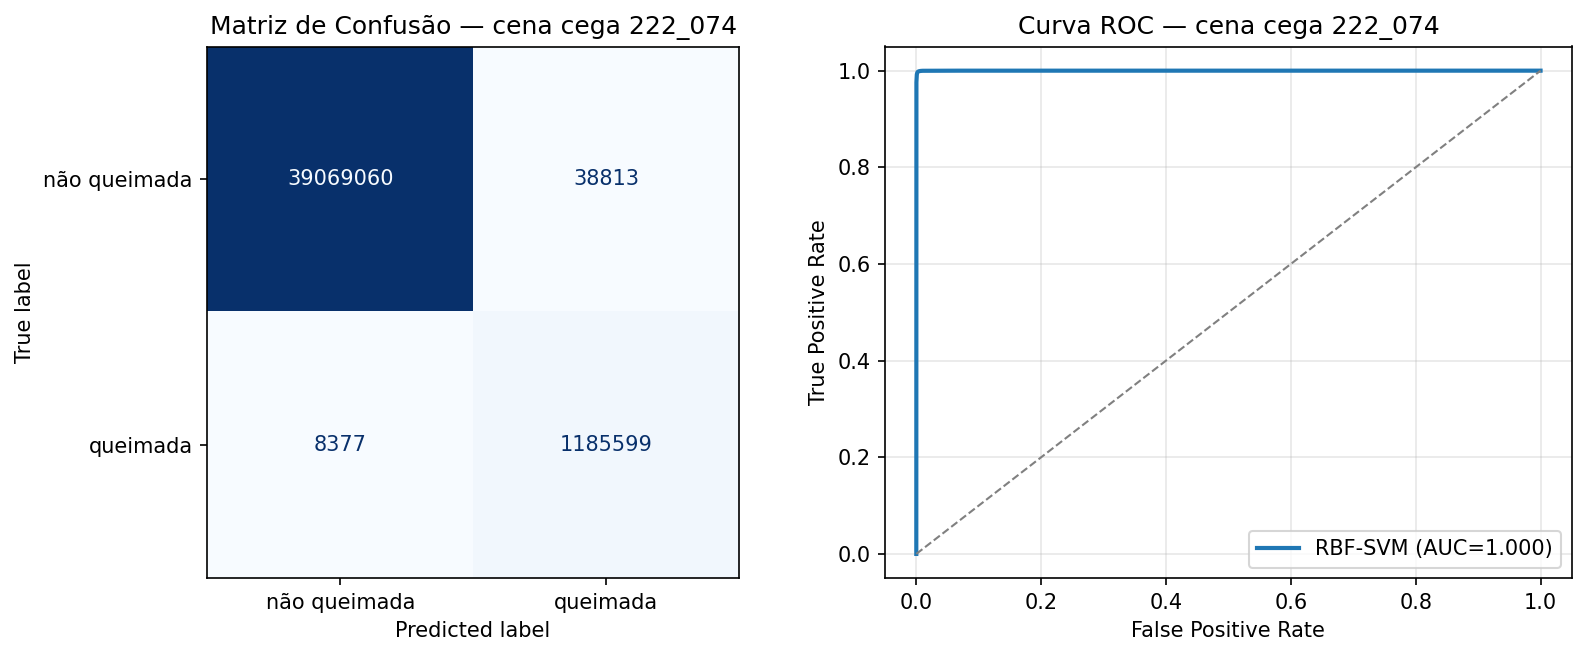
\includegraphics[width=\columnwidth]{fig_cm_222.png}
  \caption{Matrizes de confusão e curvas ROC dos testes cegos:
           cena~221\_074 — F1=99,1\% (cima) e cena~222\_074 — F1=98,1\% (baixo).
           AUC-ROC=1,000 em ambas.}
  \label{fig:cm_roc}
\end{figure}

\subsection{Vetores de Suporte}

O modelo utilizou apenas \textbf{105 vetores de suporte} — número muito
baixo para o espaço de 50~mil amostras de treino. Isso confirma que as
classes são espectralmente bem separadas: a fronteira de decisão pode ser
definida com um conjunto mínimo de exemplos representativos.

%=====================================================================
\section{Discussão}

\subsection{Alta Performance e Generalização}

Os resultados ($F_1 > 98\%$, AUC~$= 1{,}000$) demonstram que a SVM~RBF
aprendeu a identificar áreas queimadas a partir de amostras de uma única
cena e generalizou corretamente para regiões geograficamente distintas.
A estabilidade das métricas entre os dois testes cegos ($F_1 = 99{,}12\%$
e $98{,}05\%$) evidencia robustez da assinatura espectral aprendida.

\subsection{Eficiência do Kernel RBF}

A capacidade de aprender fronteiras de decisão não-lineares distingue a
SVM~RBF da versão linear. O kernel RBF possibilitou capturar relações
não-lineares entre as 10~features espectrais multitemporais, que são
determinantes para separar cicatrizes de queimada de solos expostos
e sombras.

\subsection{Limitação Principal}

A confusão entre solo exposto e cicatrizes recentes persiste como
limitação principal, problema compartilhado com métodos não
supervisionados. Ainda assim, a incorporação das imagens com nuvens como
amostras negativas mostrou-se eficaz para reduzir falsos positivos em
regiões com nebulosidade parcial.

%=====================================================================
\section{Conclusão}

A SVM~RBF aprendeu a identificar áreas queimadas a partir de amostras de
uma única cena e generalizou corretamente para regiões geograficamente
distintas, atingindo $F_1$ acima de 98\% nos dois testes cegos com
AUC-ROC perfeita. O modelo utilizou apenas \textbf{105 vetores de suporte}
— número muito baixo para o espaço de 50~mil amostras de treino —
confirmando que as classes são espectralmente bem separadas.

\begin{figure}[!t]
  \centering
  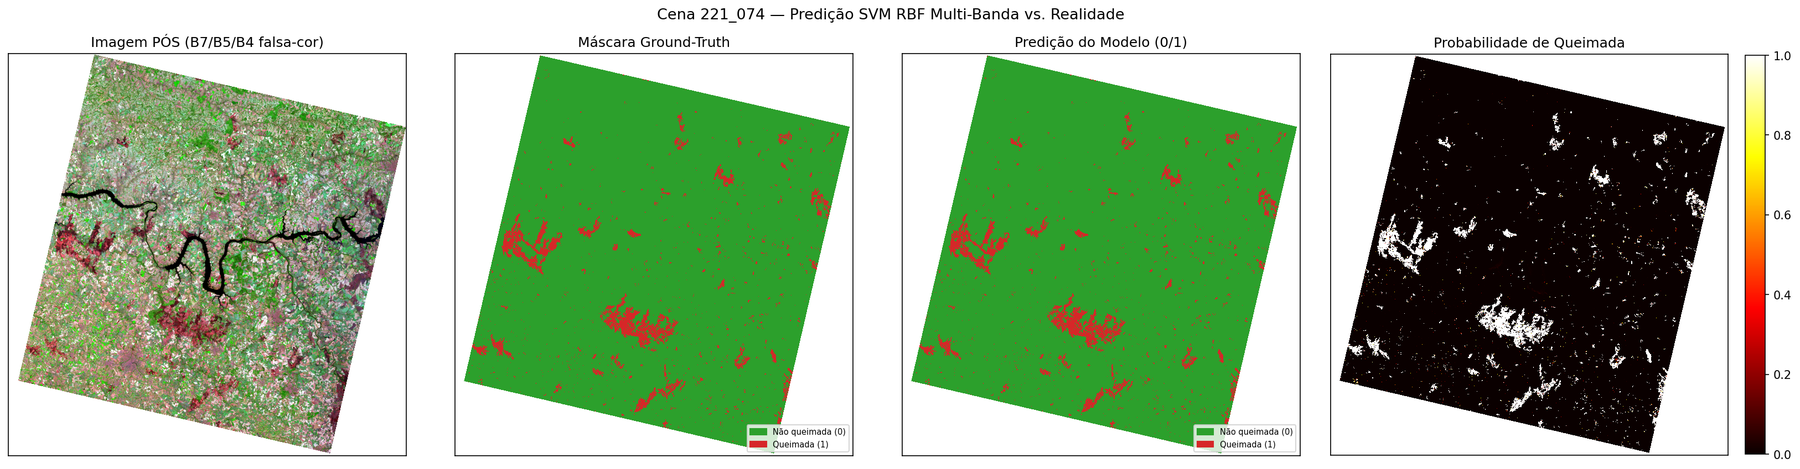
\includegraphics[width=\columnwidth]{fig_pred_221.png}\\[4pt]
  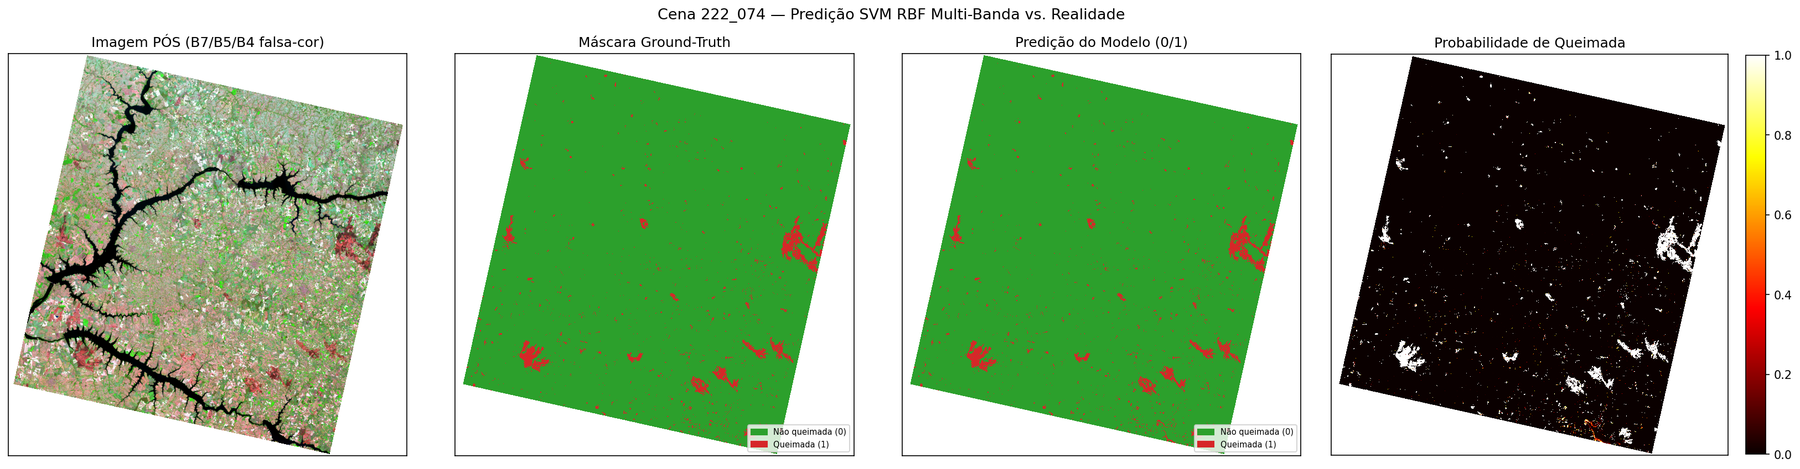
\includegraphics[width=\columnwidth]{fig_pred_222.png}
  \caption{Predição vs.\ realidade: cena~221\_074 (cima) e cena~222\_074
           (baixo). Cada linha exibe: imagem pós-queimada (falsa-cor),
           máscara \textit{ground-truth}, predição binária e mapa de
           probabilidade.}
  \label{fig:pred}
\end{figure}

A metodologia proposta demonstra que:
\begin{enumerate}
  \item a assinatura espectral multitemporal (10~features pré/pós) é
        suficientemente informativa para classificação binária robusta;
  \item a SVM~RBF com kernel Gaussiano é altamente eficiente neste domínio;
  \item a generalização entre cenas e sensores Landsat~8/9 é possível com
        treinamento em uma única cena bem representativa.
\end{enumerate}

\begin{thebibliography}{00}

\bibitem{b1}
C.~Cortes e V.~Vapnik,
``Support-vector networks,''
\textit{Machine Learning}, vol.~20, pp.~273--297, 1995.

\bibitem{b2}
C.~H.~Key e N.~C.~Benson,
``Landscape Assessment: Composite Burn Index,''
in \textit{FIREMON}, USDA Forest Service, RMRS-GTR-164-CD, 2006.

\bibitem{b3}
J.~Bergstra \textit{et al.},
``Algorithms for hyper-parameter optimization,''
\textit{NeurIPS}, vol.~24, pp.~2546--2554, 2011.

\end{thebibliography}

\end{document}
